%
% main.tex -- Paper zum Thema Optische Fouriertransformation <opt>
%
% (c) 2023 Marco Niederberger, Yanick Schoch; OST Ostschweizer Fachhochschule
%
% !TEX root = ../../buch.tex
% !TEX encoding = UTF-8
%

% TODO markings
\newcommand{\opttodo}[1] {\textbf{\textcolor{red}{TODO: #1}}}
\newcommand{\optrh}{\opttodo{REF HERE}}

\chapter{Optische Fouriertransformation\label{chapter:opt}}
\kopflinks{Optische Fouriertransformation}
\begin{refsection}
\chapterauthor{Marco Niederberger, Yanick Schoch}

Die Fouriertransformation ist in der Technik und insbesondere auch in der Elektrotechnik allgegenwärtig.
Die Berechnung wurde mehrmals verbessert und es sind diverse schnelle Algorithmen vorhanden.
Mit der optischen Fouriertransformation ist jedoch ein Werkzeug vorhanden, welches jeden aktuellen Computer überholt.

In diesem Kapitel wird gezeigt, wie aus dem physikalischen Prinzip der Beugung eine zweidimensionale Fouriertransformation entsteht.
Dabei werden zuerst die physikalischen Grundlagen erläutert und anschliessend wird das Beugungsintegral sowie dessen Näherungen hergeleitet.
Abgeschlossen wird das Kapitel mit einem praktischen Versuchsaufbau sowie einer Übersicht über mögliche Anwendungen und aktuelle Forschung.

%
% grundlagen.tex -- Paper zum Thema Optische Fouriertransformation <opt>
%
% (c) 2023 Marco Niederberger, Yanick Schoch; OST Ostschweizer Fachhochschule
%
% !TEX root = ../../buch.tex
% !TEX encoding = UTF-8
%
\section{Grundlagen\label{opt:section:grundlagen}}
\rhead{Von der Beugung zu Fourier}

\subsection{Grundlagen Wellentheorie}
Beugung kurz erklärt

\subsubsection{Fressnel / Frauhofner}
Was ist der Unterschied zwischen den beiden Approximationen?

\subsection{Herleitung}
Betrachten wir nun wie in TODO gezeigt eine unendlich dünne zylindrische Lichtquelle, welche sich axial in beide Richtingen unendlich weit erstreckt.
Allerdings muss die Quelle nicht zwingend als Lichtquelle betrachtet werden, sondern kann als eine generelle elektromagentische Quelle angesehen werden.
Dadurch kann durch anwenden der ersten Maxwellschen Gleichung
\begin{equation}
\oint_{S=\partial V} \varepsilon\vec{E}\, d\vec{S}
=
\int_{V}\rho\, dV
\end{equation}
die Elektrischefeldstärke $\vec{E}$ an jedem beliebigen Punkt in abhängigkeit des radialen Abstandes $r$ berechnet werden.
Angewendet auf die gegebene Geometrie des Zylindermantels lässt sich diese Gleichung mittels $dS = r d\varphi d\l$ als
\begin{align}
\int_{0}^{a}\int_{0}^{2\pi} \varepsilon Er\, d\varphi d\l
&=
Q
\\
2\pi r\varepsilon aE
&=
Q
\end{align}
schreiben.
Die Deckflächen konnten aufgrund der infiniten Länge des Zylinders vernachlässigt werden.
Nach der Elektrischenfeldstärke umgeformt lautet die Gleichung
\begin{equation}
E(r)
=
\frac{Q}{2\pi\varepsilon a} \cdot \frac{1}{r}
=
C \cdot \frac{1}{r}
\end{equation}
, wobei der konstante Anteil als $C$ zusammengefasst werden kann.

%
% versuch.tex -- Paper zum Thema Optische Fourier-Transformation <opt>
%
% (c) 2023 Marco Niederberger, Yanick Schoch; OST Ostschweizer Fachhochschule
%
% !TEX root = ../../buch.tex
% !TEX encoding = UTF-8
%
\section{Versuch
  \label{opt:section:versuch}}
\kopfrechts{Praktische Erprobung}

Der durchgeführte Versuch entspricht im Aufbau demjenigen aus Abbildung \ref{opt:fig:4fAufbau}.
Für die Fourier-Transformation wurden eine Linse mit 300 mm Brennweite genutzt, damit war der Effekt am besten sichtbar.
Der vorhandene Helium-Neon-Laser erzeugt einen Laserstrahl mit einem Durchmesser von $0.8$ mm.
\index{Helium-Neon-Laser}%
\index{Laser}%
Um die gerade Wellenfront in ausreichendem Durchmesser zu erhalten, wurde der Strahl mittels eines umgekehrten keplerschen Teleskops aufgeweitet.
\index{keplersches Teleskop}%
\index{Teleskop, keplersch}%
Der schematische Aufbau ist in Abbildung \ref{opt:fig:laserAufweiten} ersichtlich.
Dafür wird direkt hinter der Laserblende eine konkave Linse mit einer Brennweite $f_b = 50\,\text{mm}$ montiert 
und in einem Abstand von $f_b + f_o = 200\,\text{mm}$ eine weitere mit einer Brennweite von $f_o = 150\,\text{mm}$.
Somit wird der Laserstrahl um ein Faktor $\frac{f_o}{f_b} = 3$ vergrössert.
Dies war ausreichend, um die vorhandenen Blenden vollständig auszuleuchten.

Anschliessend konnte eine erste Blende montiert werden.
In Abbildung \ref{opt:fig:4fAufbau} ist dies als Originalbild beschrieben.
Im Abstand $f=300\,\text{mm}$ wird jetzt die erste Linse montiert und nach weiteren zwei Brennweiten die zweite Linse.
Genau in der Mitte der beiden Linsen ergibt sich die Fourier-Ebene.
Ganz am Ende des Aufbaus, eine weitere Brennweite hinter der zweiten Linse, ist das rücktransformierte Bild ersichtlich.

Im weiteren Verlauf dieses Abschnittes werden die erwarteten Ergebnisse simuliert und anschliessend mit den Beobachtungen verglichen.

\subsection{Simulation der erwarteten Ergebnissen}
Der $4f$ Versuch kann auch simuliert werden.
\index{4f Versuch@$4f$ Versuch}%
In unserem Fall geschah dies mit \emph{Python} und der \emph{numpy} Bibliothek.
\index{numpy}%
\index{Python}%
Zuerst wird ein Input-Bild erstellt, welches anschliessend bearbeitet wird.
Als Input wurden ein Dreifachspalt sowie ein Gitter verwendet.
Mittels zweidimensionaler diskreter Fast-Fourier-Transformation (FFT) wird das Originalbild in den Frequenzbereich transformiert.
Anschliessend kann dies mit einem digitalen Filter gefiltert werden.
Die Filter werden so ausgeführt, wie sie in Abbildung \ref{opt:fig:filterarten} aufgeführt sind.
Das bedeutet, dass zum Beispiel ein Tiefpass einen runden Durchlassbereich um den Nullpunkt hat.
Schlussendlich wird das gefilterte Frequenzspektrum mittels zweidimensionaler FFT wieder rücktransformiert.
Abbildung \ref{opt:fig:three_slit_simulation} zeigt diesen Vorgang am Beispiel eines Dreifachspalts und 
in Abbildung \ref{opt:fig:grid_simulation} wird dasselbe mit einem Gitter simuliert.

Die verwendeten Python-Skripte der Simulation sind im Repository des Buches\footnote{\url{https://github.com/AndreasFMueller/SeminarHarmonischeAnalysis/tree/master/buch/papers/opt/code}}
abgelegt.

\subsection{Versuchsdurchführung}
Zuerst wurde die Funktion des Aufbaus mit einem $2f$ Versuch verifiziert.
Dabei wird nur eine Linse aus dem $4f$ Aufbau verwendet und das entstandene Spektrum wird im Abstand der Brennweite betrachtet.
Die dabei entstandenen Bilder entsprachen den Erwartungen.
Für den Einzelspalt war, wie in Abschnitt \ref{opt:sec:exampleSingleSlit} berechnet, eine sinc-förmige Verteilung der Intensität zu betrachten.

Nach dieser Verifizierung wurde die zweite Linse ebenfalls montiert und die Abbildungsebene hinter die zweite Linse gelegt.
Beim Dreifachspalt konnte die Fourier-Transformation und Rücktransformation erfolgreich ausgeführt werden.
Die Filterung mittels eines optischen Tiefpasses konnte jedoch nicht nachgebildet werden.
Der genaue Grund dafür konnte nicht eruiert werden.
Mögliche Ursachen sind eine zu grosse Blende, eine nicht optimale Ausrichtung der optischen Achse oder eine zu geringe Auflösung der Auswerteeinheit.

\subsection{Vergleich der Simulation}
In der Abbildung \ref{opt:fig:experiment} sind die Resultate aus dem Versuch mit dem Dreifachspalt ersichtlich.
Wenn das erhaltene Spektrum mit demjenigen aus der Simulation in Abbildung \ref{opt:fig:three_slit_simulation} verglichen wird, ist eine Übereinstimmung ersichtlich.
In beiden Fällen ist auf der $x$-Achse eine erhöhte Intensität zu beobachten mit einem grossen Anteil im Ursprung.
Ebenfalls in beiden Fällen kann auch auf der $y$-Achse eine kleine Intensität beobachtet werden.
Diese folgt davon, dass der Spalt eine beschränkte Dimension in der $y$-Richtung hat und somit auch dort die Welle gebeugt wird.
Beim reellen Versuch können noch weitere Bereiche mit einer sichtbaren Intensität ausgemacht werden, welche in der Simulation nicht ersichtlich sind.
Dies war jedoch zu erwarten, da die Simulation im Gegensatz zum realen Versuchsaufbau viel genauer ist und sich nicht durch Störungen im Aufbau beeinflussen lässt.


\begin{figure}
    \centering
    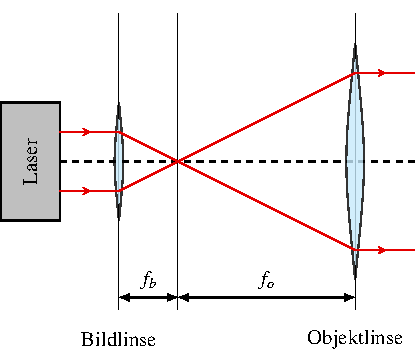
\includegraphics[width=60mm]{papers/opt/images/laserAufweiten.pdf}
    \caption{Die Vergrösserung des Laserlichts erfolgt mit einem Kepler-Teleskop.
        Dazu werden zwei Linsen mit unterschiedlichen Brennweiten verwendet.
\index{keplersches Teleskop}%
        Der Abstand dazwischen ist die Summe der beiden Brennweiten.}
    \label{opt:fig:laserAufweiten}
\end{figure}

\begin{figure}
    \centering
    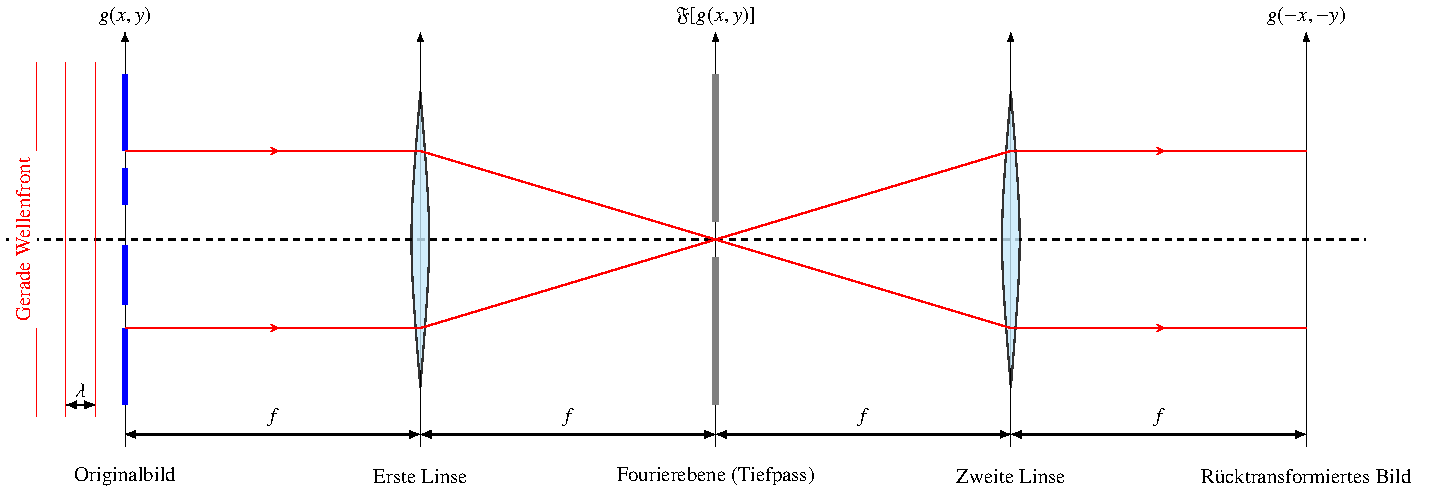
\includegraphics[width=\textwidth]{papers/opt/images/4fAufbau.pdf}
    \caption{Der $4f$ Aufbau ermöglicht eine Fourier-Transformation des Originalbildes sowie eine Rücktransformation aus der Fourier-Ebene.
\index{Fourier-Ebene}%
    In dieser Abbildung wird die transformierte Funktion mit einem Tiefpass gefiltert.
\index{Tiefpass}%
    Weitere Details zu den Filtern folgen im Abschnitt \ref{opt:section:filter}.}
    \label{opt:fig:4fAufbau}
\end{figure}

\begin{figure}
    \centering
    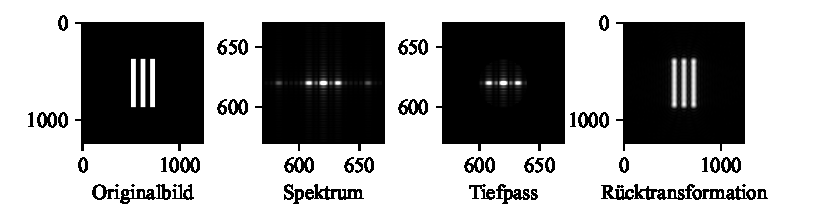
\includegraphics[width=\textwidth]{papers/opt/images/dreifachspalt_tiefpass.pdf}
    \caption{Der Dreifachspalt wird zunächst fouriertransformiert, dann mit einem Tiefpass gefiltert und wieder rücktransformiert.
    Die ursprünglich scharfen Kanten des Spalts werden dadurch unscharf wiedergegeben.}
    \label{opt:fig:three_slit_simulation}
\end{figure}

\begin{figure}
    \centering
    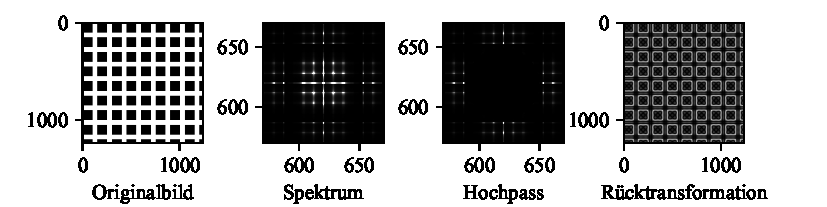
\includegraphics[width=\textwidth]{papers/opt/images/gitter_hochpass.pdf}
    \caption{Das Gitter wird zunächst fouriertransformiert, dann mit einem Hochpass gefiltert und wieder rücktransformiert.
    In der Rücktransformation sind insbesondere die harten Kanten des Gitters erkennbar.}
    \label{opt:fig:grid_simulation}
\end{figure}

\begin{figure}
    \centering
    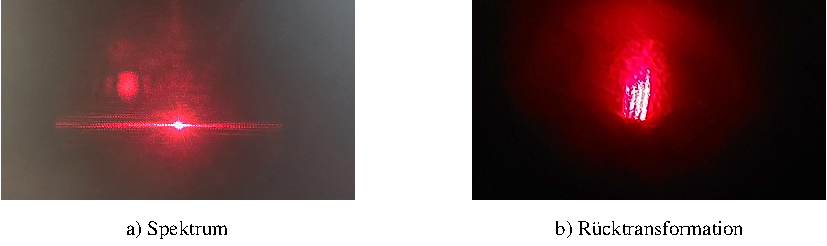
\includegraphics[width=\textwidth]{papers/opt/images/experiment.pdf}
    \caption{Der $4f$ Versuch aus dem Abschnitt \ref{opt:section:versuch} wurde hier mit einem Dreifachspalt durchgeführt.
    Abbildung a) zeigt das daraus entstandene Spektrum und in der Abbildung b) ist die Rücktransformation davon zu sehen.}
    \label{opt:fig:experiment}
\end{figure}

%
% anwendungen.tex -- Paper zum Thema Optische Fouriertransformation <opt>
%
% (c) 2023 Marco Niederberger, Yanick Schoch; OST Ostschweizer Fachhochschule
%
% !TEX root = ../../buch.tex
% !TEX encoding = UTF-8
%
\section{Anwendungen
  \label{opt:section:anwendungen}}
\rhead{Praktische Anwendungen}

\subsection{Mustererkennung}
Die schnelle Erstellung einer Fouriertransformation kann für die Erkennung von vordefinierten Mustern verwendet werden.
\opttodo{Add skizze}
Dabei wird das zu untersuchende Muster auf die Bildebene der ersten Linse gelegt \opttodo{Ref zu Bild}.
In der Fourierebene wird dann die bekannte Fouriertransformation des gesuchten Musters montiert.
Diese Maske ist bei den gewünschten Frequenzanteilen durchlässig, an allen anderen Orten lichtundurchlässig.
Mittels einer einfachen Helligkeitsmessung mithilfe einer Photodiode kann anschliessend auf das gesuchte Muster geschlossen werden.
In \cite{opt:YT:PatternRecognition} wird dies anhand eines Versuches mit den Buchstaben A und B visualisiert.
Die Geschwindigkeit hierbei ist nicht mehr durch eine elektronische Schaltung gegeben.
Einzig limitierend ist die Geschwindigkeit, mit der das Licht durch den Versuchsaufbau gelangt plus die Anstiegszeit der Photodiode.
Abgeschätzt mit einer Distanz von 20 cm und einer Anstiegszeit von 100 ps liegt die totale Zeit pro Erkennung bei rund 900 ps.
Dies entspricht einer Frequenz im Bereich von 1 GHz, mit welcher Muster erkennt werden können.

\begin{figure}
    \centering
    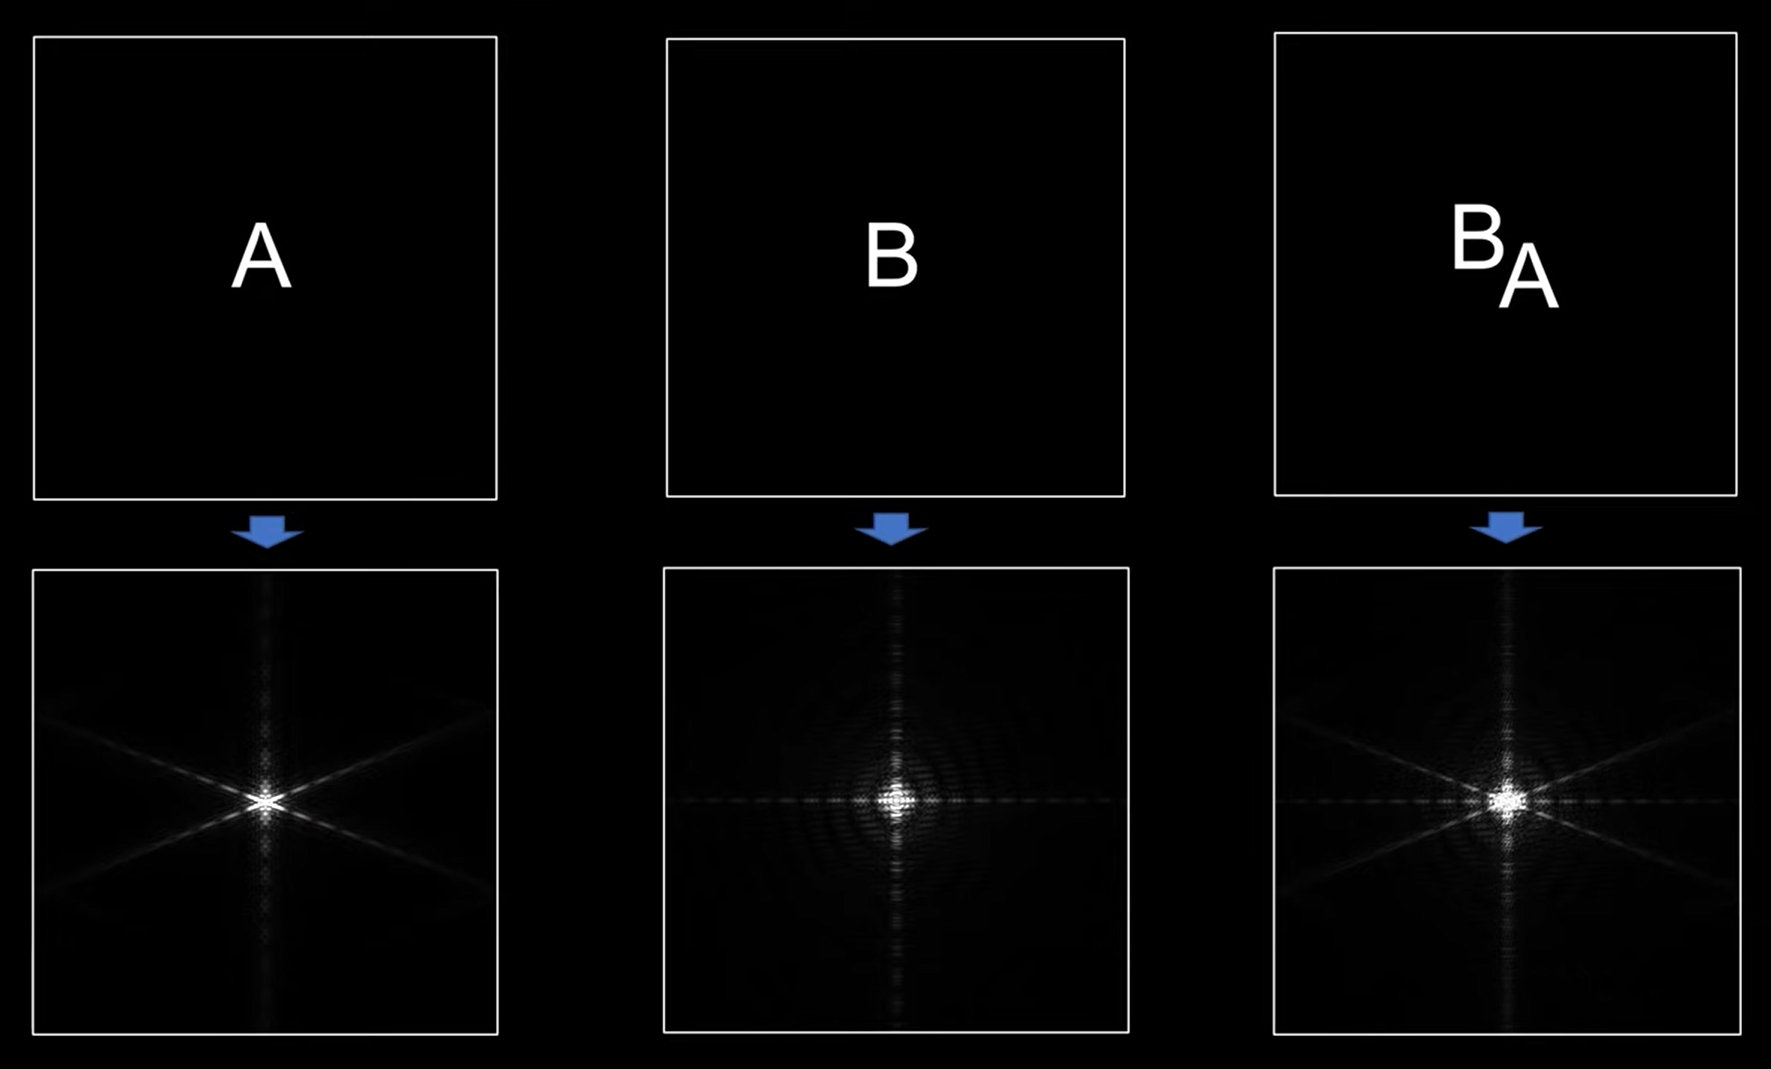
\includegraphics[width=0.6\textwidth]{papers/opt/images/pattern_YT.png}
    \label{opt:fig:patternYT}
    \caption{Frequenzspektrum der verschiedenen Muster. 
    Mittels einer Maskierung und einer Helligkeitsmessung kann das entsprechende Muster detektiert werden.}
\end{figure}
\opttodo{Add sketch with character A and B after fouriermask}

\subsection{Diffractive deep neural network}
Beim obenstehenden Beispiel wurde nur mit einer einzelnen Blende gearbeitet, um das gesuchte Muster zu erkennen.
In \cite{opt:Lin.2018} wurde dieser Ansatz durch Xing et al. erweitert und mit mehreren Ebenen erfolgreich getestet.
Abbildung \ref{opt:fig:handwriting}a zeigt den schematische Aufbau mit fünf Ebenen.
Der Grundsatz bleibt gleich; koheräntes Licht wird von einer ersten Input Ebene gebogen und anschliessend an fünf weiteren Ebenen.
Dies entspricht im Ansatz den verschiedenen Verknüpften Neutronen eines neuronalen Netzwerkes.
Nach den Beugungsebenen wird das Licht durch mehrere Detektoren erkannt.
Xing et al. konnten somit erfolgreich handschriftliche Zahlen detektieren.
Mittels fünf aufeinanderfolgenden Ebenen und zehn Detektoren gelang es ihnen, mehr als 90\% der Schriften korrekt zuzuordnen.

\begin{figure}
    \centering
    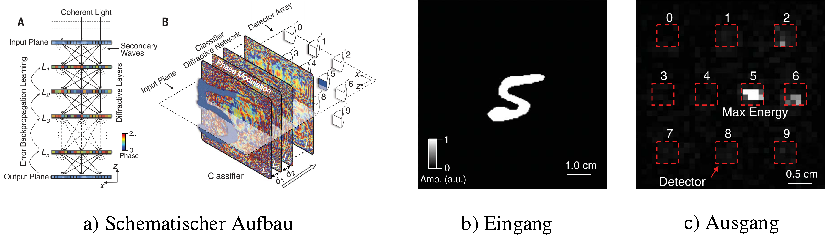
\includegraphics[width=\textwidth]{papers/opt/images/handwriting.pdf}
    \caption{Abbildung a) zeigt den Aufbau, wie er in \cite{opt:Lin.2018} verwendet wurde, um handschriftliche Ziffern zu erkennen.
    Abbildung b) und c) zeigen den Eingang sowie das Bild auf dem Detektor des Systems}
    \label{opt:fig:handwriting}
\end{figure}

\subsection{Aktuelle Forschung im Bereich Photonics}
\opttodo{Add infos from OST - Photonics}

\subsection{James-Webb-Weltraumteleskop}
Eine weiteres Beispiel der Beugung befindet sich aktuell im Weltraum.
Auf den Bildern des James-Webb-Weltraumteleskop (JWST) sind jeweils sechs (beziehungsweise drei) helle Strahlen ersichtlich.
Diese werden durch die Geometrie des Spiegels erzeugt.

Das Teleskop besteht aus einem sechseckigen Hauptspiegel mit einem Loch sowie einem vorgelagerten Spiegel.
Dieser wiederum ist mit drei Stützen mit der Struktur des JWST verbunden.
Dabei wurden zwei Stützen so platziert, dass deren Strahlen deckungsgleich mit denjenigen des Hauptspiegels sind.
Die dritte Stütze ist senkrecht montiert und somit nicht mit einem Strahl des Hauptspiegels deckungsgleich.
Dies ist auf den Bildern als vierter Strahl zu sehen.
Zusammen ergeben diese beiden Effekte in Abbildung \ref{opt:fig:jwst} die charakteristischen Strahlen, welche auf
den veröffentlichten Bildern des JWST zu sehen sind.

\begin{figure}
    \centering

    \subfigure{
        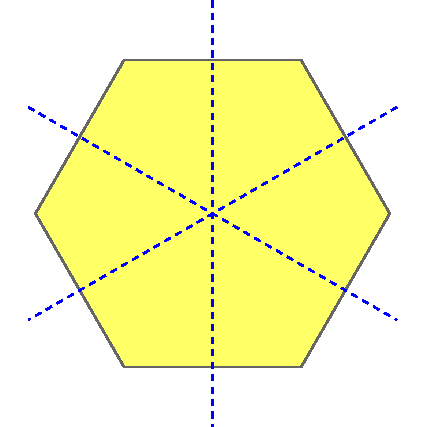
\includegraphics[page=1, width=0.3\linewidth]{papers/opt/images/jwst_sechseck.pdf}
    }
    \hfill
    \subfigure{
        \includegraphics[page=2, width=0.3\linewidth]{papers/opt/images/jwst_sechseck.pdf}
    }
    \hfill
    \subfigure{
        
\includegraphics[width=0.3\linewidth]{papers/opt/images/jamesWebb_cropped_publicDomain.png}
    }
    \caption{Links die Strahlen der sechs Aussenkanten, mittig der drei Stützen sowie rechts eine Aufnahme der NASA (Public Domain)
        des James-Webb-Weltraumteleskop mit den charakteristischen Strahlen.}
    \label{opt:fig:jwst}
\end{figure}

%
% filter.tex -- Paper zum Thema Optische Fouriertransformation <opt>
%
% (c) 2023 Marco Niederberger, Yanick Schoch; OST Ostschweizer Fachhochschule
%
% !TEX root = ../../buch.tex
% !TEX encoding = UTF-8
%
\section{Filter
\label{opt:section:filter}}
\rhead{Filterdesign}

Auch bei der optischen Fouriertransformation kann das Signal anschliessend in der Fourierebene bearbeitet werden.
Im optischen entspricht dies einer Blende.
Diese wird, wie in Abbildung \ref{opt:fig:4fAufbau} gezeigt, zwischen den beiden Linsen platziert.
Typische Filter in der Elektrotechnik sind Tiefpass, Hochpass, Bandpass und Bandsperre.
Deren Realisierung in der Optik ist in Abbildung \ref{opt:fig:filterarten} ersichtlich.

Im Nullpunkt der Filterebene sind die tiefen Frequenzen (DC-Anteil) und entlang der Achsen die höheren Frequenzen zu erkennen.
Somit entspricht eine lichtundurchlässige Fläche mit einem Loch in der Mitte einem Tiefpass und eine lichtundurchlässige Scheibe einem Hochpass.
Nach diesem Prinzip lassen sich auch die weiteren typischen Filter realisieren.

\begin{figure}
    \centering
    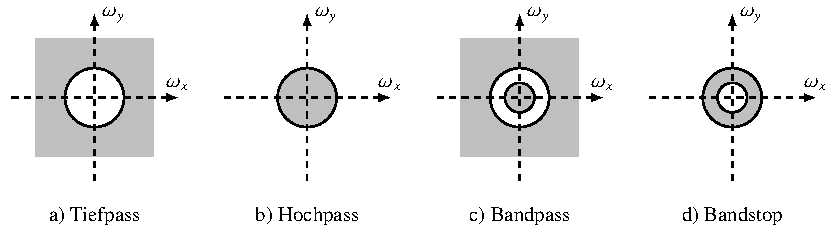
\includegraphics[width=\textwidth]{papers/opt/images/filterarten.pdf}

    \caption{Realisierung typischer Filter als optische Systeme;
        wobei grau lichtundurchlässig und weiss lichtdurchlässig bedeutet.}
    \label{opt:fig:filterarten}
\end{figure}

\subsection{Anwendung in der Bildverarbeitung}
\label{opt:section:image_processing}

Wie in Kapitel \ref{opt:section:filter} gezeigt kann in der Fourierebene gefiltert werden.
Im folgenden wird dies an einem Bild und mehreren Filtern illustriert.
In Abbildung \ref{opt:fig:image_raw} ist das Originalbild sowie dessen Fouriertransformation zu sehen.
Dabei entspricht die Farbe weiss im Spektrum einer hohen Energie und die Farbe schwarz einer tiefen Energie.

Das besagte Spektrum wird in Abbildung \ref{opt:fig:image_lowpass} mit einem Tiefpass gefiltert.
Wie bereits erwähnt entspricht ein Tiefpass im Optischen einer Blende, welche alles Licht ausserhalb eines Kreises blockiert.
Das so entstehende Spektrum wird rücktransformiert und führt zu einer verwaschenen Kopie des Originalbildes.

Abbildung \ref{opt:fig:image_highpass} zeigt genau das Gegenteil. 
Das Spektrum wird mittels Hochpass gefiltert, das bedeutet, dass eine Kreisfläche geblockt und alles andere durchgelassen wird.
Die Rücktransformation dieser Filterung betont die scharfen Kanten des Originalbildes. 

\begin{figure}
    \centering
    \subfigure{
        \includegraphics[width=0.4\textwidth]{../../Optical_Fourier/python_fft2d/output/image.png}
    }
    \subfigure{
        \includegraphics[width=0.4\textwidth]{../../Optical_Fourier/python_fft2d/output/image_fourier.png}
    }

    \caption{Beispielbild und dessen Fouriertransformation}
    \label{opt:fig:image_raw}
\end{figure}

\begin{figure}
    \centering
    \subfigure{
        \includegraphics[width=0.4\textwidth]{../../Optical_Fourier/python_fft2d/output/image_fourier_lowpass.png}
    }
    \subfigure{
        \includegraphics[width=0.4\textwidth]{../../Optical_Fourier/python_fft2d/output/image_reconstructed_lowpass.png}
    }

    \caption{Das Spektrum aus Abbildung \ref{opt:fig:image_raw} wird mit einem Tiefpass gefiltert und wieder rücktransformiert.
    Das rücktransformierte Bild ergibt eine verwaschene Kopie des Originalbildes.}
    \label{opt:fig:image_lowpass}
\end{figure}

\begin{figure}
    \centering
    \subfigure{
        \includegraphics[width=0.4\textwidth]{../../Optical_Fourier/python_fft2d/output/image_fourier_highpass.png}
    }
    \subfigure{
        \includegraphics[width=0.4\textwidth]{../../Optical_Fourier/python_fft2d/output/image_reconstructed_highpass.png}
    }

    \caption{Das Spektrum aus Abbildung \ref{opt:fig:image_raw} wird mit einem Hochpass gefiltert und wieder rücktransformiert.
    Das rücktransformierte Bild betont die harten Kanten im Originalbild.}
    \label{opt:fig:image_highpass}
\end{figure}

\subsection{Vergleich mit Filter 1. / 2. Ordnung}

\subsection{Cutoff Frequenz, Abfall nach $\omega_c$}

\subsection{Wo ist welche Frequenz $Hz <=> mm$ auf der Fourierebene}
Evt Formel in Abhängigkeit von der Wellenlänge, Distanz und Brennweite



\printbibliography[heading=subbibliography]
\end{refsection}
